\chapter{CSS Fondamentale}
\label{cap:css_base}

\section{Cos'è CSS?}

CSS (Cascading Style Sheets) è usato per stilizzare gli elementi HTML. Mentre HTML (\ref{cap:intro_html}) descrive la struttura, CSS controlla l'aspetto visivo.

\section{Selettori CSS}

I selettori CSS identificano quali elementi stilizzare:

\begin{lstlisting}[language=CSS]
/* Selettore elemento */
p { color: blue; }

/* Selettore classe */
.highlight { background: yellow; }

/* Selettore ID */
#header { margin: 0; }

/* Selettore attributo */
input[type="email"] { border: 1px solid blue; }

/* Combinatori */
div p { color: red; }        /* Discendente */
div > p { color: green; }    /* Figlio diretto */
h1 + p { color: gray; }      /* Elemento adiacente */
\end{lstlisting}

\section{Specificity}

La specificity determina quale regola CSS ha priorità quando più regole si applicano allo stesso elemento:

\begin{lstlisting}[language=CSS]
/* Specificity: 0,0,1 */
p { color: blue; }

/* Specificity: 0,1,0 */
.class { color: green; }

/* Specificity: 0,1,1 */
p.class { color: red; }

/* Specificity: 1,0,0 */
#id { color: yellow; }
\end{lstlisting}

\subsection{Piramide della Specificity}

La specificity può essere visualizzata come una piramide, dove i livelli superiori hanno precedenza sui livelli inferiori:

\begin{center}
\begin{tikzpicture}[scale=0.9]
    % Definisci gli stili
    \tikzstyle{level}=[trapezium, trapezium left angle=70, trapezium right angle=110,
                       draw=black, thick, minimum height=1cm, align=center]

    % !important (livello massimo)
    \node[level, fill=red!60, minimum width=3cm, font=\small\bfseries] (important) at (0,5) {
        !important\\
        \footnotesize Peso: $\infty$
    };

    % Inline styles
    \node[level, fill=orange!50, minimum width=4.5cm, font=\small\bfseries, below=0.8cm of important] (inline) {
        Inline Styles\\
        \footnotesize (1,0,0,0)
    };

    % ID selectors
    \node[level, fill=yellow!60, minimum width=6cm, font=\small\bfseries, below=0.8cm of inline] (id) {
        ID Selectors\\
        \footnotesize \texttt{\#header} (0,1,0,0)
    };

    % Class, attribute, pseudo-class
    \node[level, fill=green!40, minimum width=7.5cm, font=\small, below=0.8cm of id] (class) {
        \textbf{Class, Attribute, Pseudo-class}\\
        \footnotesize \texttt{.btn}, \texttt{[type="text"]}, \texttt{:hover} (0,0,1,0)
    };

    % Element, pseudo-element
    \node[level, fill=blue!30, minimum width=9cm, font=\small, below=0.8cm of class] (element) {
        \textbf{Element \& Pseudo-element}\\
        \footnotesize \texttt{div}, \texttt{p}, \texttt{::before} (0,0,0,1)
    };

    % Universal selector
    \node[rectangle, draw=black, thick, fill=gray!20, minimum width=10cm, minimum height=0.7cm,
          font=\small, below=0.8cm of element] (universal) {
        \textbf{Universal Selector} \texttt{*} (0,0,0,0)
    };

    % Freccia indicatore priorità
    \draw[->, ultra thick, red!70] (-6,5.5) -- (-6,1) node[midway, left, align=center, font=\footnotesize] {
        Priorità\\crescente\\$\uparrow$
    };
\end{tikzpicture}
\end{center}

\subsection{Come si calcola la specificity}

La specificity si rappresenta come una tupla $(a, b, c, d)$ dove ogni posizione conta un tipo diverso di selettore. Il valore \textbf{a} rappresenta il numero di inline styles (attributi \texttt{style="..."}), che hanno la massima priorità. Il valore \textbf{b} conta il numero di ID selectors (\texttt{\#id}), che sono altamente specifici. Il valore \textbf{c} include il numero di class selectors, attribute selectors e pseudo-classes, che hanno una priorità media. Infine, il valore \textbf{d} conta il numero di element selectors e pseudo-elements, che hanno la priorità più bassa tra i selettori normali.

\textbf{Esempi di calcolo}:

\begin{lstlisting}[language=CSS]
/* (0,0,0,1) */
p { color: blue; }

/* (0,0,1,0) */
.highlight { color: green; }

/* (0,0,1,1) */
p.highlight { color: red; }

/* (0,1,0,0) */
#main { color: orange; }

/* (0,1,2,1) */
#main .content p.intro { color: purple; }

/* (1,0,0,0) */
<p style="color: pink;">Inline</p>
\end{lstlisting}

\begin{attenzione}
Quando due regole hanno la stessa specificity, vince quella dichiarata per ultima nel CSS. Il selettore universale \texttt{*} ha specificity (0,0,0,0) e non influenza il calcolo.
\end{attenzione}

\begin{nota}
Regola generale della specificity: \texttt{!important} > Inline > ID > Class > Element. Evita \texttt{!important} quando possibile perché rende il CSS difficile da mantenere.
\end{nota}

\section{Box model}

Ogni elemento HTML è un rettangolo composto da:

\begin{lstlisting}[language=CSS]
div {
  width: 300px;
  height: 200px;
  padding: 20px;        /* Spazio interno */
  border: 2px solid;    /* Bordo */
  margin: 10px;         /* Spazio esterno */
  box-sizing: border-box;
}
\end{lstlisting}

\subsection{Componenti del box model}

\begin{description}
  \item[Content] Area con il contenuto
  \item[Padding] Spazio interno tra content e border
  \item[Border] Linea intorno al padding
  \item[Margin] Spazio esterno tra border e elementi vicini
\end{description}

\begin{center}
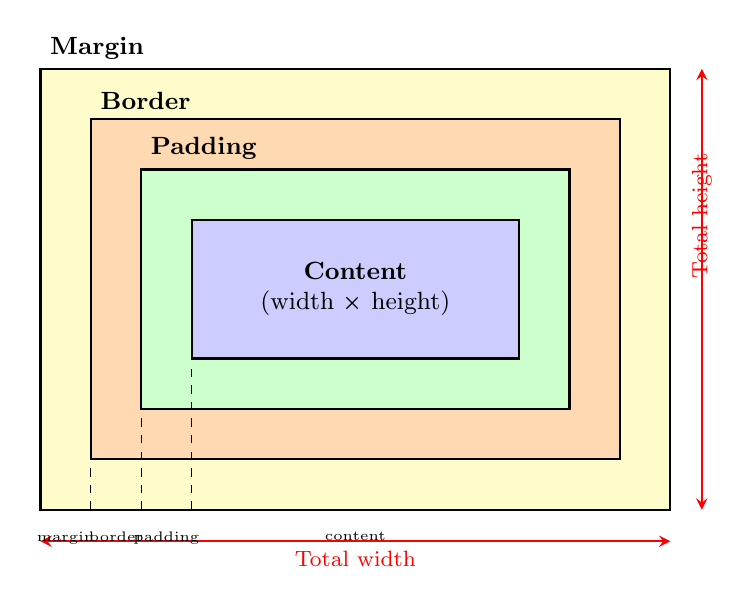
\begin{tikzpicture}[scale=0.8]
    % Margin (esterno)
    \draw[fill=yellow!20, draw=black, thick] (0,0) rectangle (10,7);
    \node[above right, font=\small\bfseries] at (0,7) {Margin};

    % Border
    \draw[fill=orange!30, draw=black, thick] (0.8,0.8) rectangle (9.2,6.2);
    \node[above right, font=\small\bfseries] at (0.8,6.2) {Border};

    % Padding
    \draw[fill=green!20, draw=black, thick] (1.6,1.6) rectangle (8.4,5.4);
    \node[above right, font=\small\bfseries] at (1.6,5.4) {Padding};

    % Content
    \draw[fill=blue!20, draw=black, thick] (2.4,2.4) rectangle (7.6,4.6);
    \node[align=center, font=\small] at (5,3.5) {\textbf{Content}\\(width × height)};

    % Frecce dimensioni
    \draw[<->, >=stealth, thick, red] (0,-0.5) -- node[below, font=\footnotesize] {Total width} (10,-0.5);
    \draw[<->, >=stealth, thick, red] (10.5,0) -- node[right, font=\footnotesize, rotate=90] {Total height} (10.5,7);

    % Annotazioni
    \draw[dashed] (0.8,0) -- (0.8,0.8);
    \draw[dashed] (1.6,0) -- (1.6,1.6);
    \draw[dashed] (2.4,0) -- (2.4,2.4);

    \node[below, font=\tiny] at (0.4,-0.2) {margin};
    \node[below, font=\tiny] at (1.2,-0.2) {border};
    \node[below, font=\tiny] at (2,-0.2) {padding};
    \node[below, font=\tiny] at (5,-0.2) {content};
\end{tikzpicture}
\end{center}

\textbf{Calcolo dimensioni totali}:
Il calcolo delle dimensioni totali di un elemento dipende dal valore della proprietà \texttt{box-sizing}. Con \texttt{content-box} (il valore di default), la larghezza totale si calcola sommando width, padding, border e margin, il che significa che specificare una width di 300px risulterà in un elemento effettivamente più largo una volta aggiunti padding, border e margin. Al contrario, con \texttt{border-box}, la larghezza totale include già padding e border all'interno del valore di width specificato, escludendo solo il margin. Questo rende \texttt{border-box} molto più intuitivo perché il valore di width che specifichi corrisponde alla dimensione visibile dell'elemento, border incluso.

\begin{lstlisting}[language=CSS]
/* content-box (default): width = solo content */
div {
  width: 300px;      /* Solo content */
  padding: 20px;     /* +40px */
  border: 5px;       /* +10px */
  margin: 10px;      /* +20px */
  /* Total width = 300 + 40 + 10 + 20 = 370px */
}

/* border-box: width = content + padding + border */
div {
  box-sizing: border-box;
  width: 300px;      /* Include padding e border */
  padding: 20px;     /* Già incluso */
  border: 5px;       /* Già incluso */
  margin: 10px;      /* +20px */
  /* Total width = 300 + 20 = 320px */
  /* Content width = 300 - 40 - 10 = 250px */
}
\end{lstlisting}

\begin{attenzione}
Usa \texttt{box-sizing: border-box} per calcoli più intuitivi. Molti framework CSS (Bootstrap, Tailwind) lo impostano di default con:
\begin{lstlisting}[language=CSS]
*, *::before, *::after {
  box-sizing: border-box;
}
\end{lstlisting}
\end{attenzione}

\section{Proprietà CSS comuni}

\begin{itemize}
  \item \texttt{color}: Colore del testo
  \item \texttt{background-color}: Colore sfondo
  \item \texttt{font-size}: Dimensione font
  \item \texttt{text-align}: Allineamento testo (left, center, right, justify)
  \item \texttt{display}: Tipo di visualizzazione (block, inline, flex, grid)
  \item \texttt{width}, \texttt{height}: Dimensioni elemento
  \item \texttt{border}: Bordo elemento
  \item \texttt{box-shadow}: Ombra elemento
\end{itemize}

\section{Unità di misura}

\begin{description}
  \item[px] Pixel (unità assoluta, non scalare)
  \item[em] Relativo alla font-size del genitore
  \item[rem] Relativo alla font-size dell'elemento radice (html)
  \item[\%] Percentuale del genitore
  \item[vw/vh] Viewport width/height (schermo utente)
\end{description}

\begin{attenzione}
Preferisci \texttt{rem} e \texttt{\%} a \texttt{px} per layout più responsive e accessibili.
\end{attenzione}

\section{Esercizi}

\subsection{Esercizio 1 (Base)}
Calcola la specificity di vari selettori CSS. Dato: \texttt{div.card p.text}, \texttt{\#header .nav}, \texttt{p}, \texttt{.class} - classifica per specificity.

\subsection{Esercizio 2 (Intermedio)}
Crea una pagina stilizzata usando selettori diversi e proprietà box model. Includi: colori, padding, margin, border, width.

\subsection{Esercizio 3 (Avanzato)}
Crea un layout complesso usando CSS senza framework. Includi: card, header, navigation bar, footer con stili responsive.

\section{Esercizio Pratico Completo: Card Portfolio}

Crea una pagina con card stilizzate per mostrare progetti personali.

\subsection{Requisiti}

\begin{itemize}
  \item 3 card con: immagine, titolo, descrizione, link
  \item Card hanno padding, border, box-shadow
  \item Responsive: ridimensionati per mobile
  \item Colori coerenti
  \item Hover effects (bonus)
\end{itemize}

\subsection{Soluzione HTML}

\begin{lstlisting}[language=HTML]
<!DOCTYPE html>
<html lang="it">
<head>
  <meta charset="UTF-8" />
  <meta name="viewport" content="width=device-width, initial-scale=1.0" />
  <title>Portfolio</title>
  <link rel="stylesheet" href="style.css" />
</head>
<body>
  <div class="container">
    <h1>Miei Progetti</h1>

    <div class="card">
      <img src="project1.jpg" alt="Progetto 1">
      <div class="card-content">
        <h2>Sito di Vendita</h2>
        <p>Un e-commerce moderno con Flexbox e Grid</p>
        <a href="/progetti/ecommerce.html" class="btn">Visualizza</a>
      </div>
    </div>

    <div class="card">
      <img src="project2.jpg" alt="Progetto 2">
      <div class="card-content">
        <h2>Blog Responsivo</h2>
        <p>Blog con SCSS e media queries</p>
        <a href="/progetti/blog/index.html" class="btn">Visualizza</a>
      </div>
    </div>

    <div class="card">
      <img src="project3.jpg" alt="Progetto 3">
      <div class="card-content">
        <h2>App Todo</h2>
        <p>Todo list con JavaScript puro</p>
        <a href="/progetti/todo-app/demo.html" class="btn">Visualizza</a>
      </div>
    </div>
  </div>
</body>
</html>
\end{lstlisting}

\subsection{Soluzione CSS (style.css)}

\begin{lstlisting}[language=CSS]
/* Reset */
* {
  margin: 0;
  padding: 0;
  box-sizing: border-box;
}

body {
  font-family: Arial, sans-serif;
  background-color: #f5f5f5;
  padding: 20px;
}

.container {
  max-width: 1200px;
  margin: 0 auto;
}

h1 {
  text-align: center;
  margin-bottom: 40px;
  color: #333;
}

/* Card styling */
.card {
  background-color: white;
  border-radius: 8px;
  overflow: hidden;
  box-shadow: 0 2px 10px rgba(0, 0, 0, 0.1);
  margin-bottom: 20px;
  transition: transform 0.3s ease;
}

.card:hover {
  transform: translateY(-5px);
  box-shadow: 0 5px 20px rgba(0, 0, 0, 0.2);
}

.card img {
  width: 100%;
  height: 250px;
  object-fit: cover;
}

.card-content {
  padding: 20px;
}

.card h2 {
  color: #333;
  margin-bottom: 10px;
}

.card p {
  color: #666;
  margin-bottom: 15px;
  line-height: 1.5;
}

.btn {
  display: inline-block;
  padding: 10px 20px;
  background-color: #007bff;
  color: white;
  text-decoration: none;
  border-radius: 4px;
  transition: background-color 0.3s;
}

.btn:hover {
  background-color: #0056b3;
}

/* Responsive per mobile */
@media (max-width: 768px) {
  .container {
    padding: 0;
  }

  h1 {
    font-size: 1.5rem;
  }

  .card {
    margin-bottom: 15px;
  }
}
\end{lstlisting}

\subsection{Spiegazione Dettagliata}

\subsubsection{Reset CSS}
\texttt{* { margin: 0; padding: 0; }} rimuove margini/padding di default del browser. \texttt{box-sizing: border-box} fa sì che padding/border siano inclusi nella larghezza.

\subsubsection{Card Styling}
\begin{itemize}
  \item \texttt{border-radius: 8px} arrotonda gli angoli
  \item \texttt{box-shadow} crea ombra sottile (4 valori: offset-x, offset-y, blur, color)
  \item \texttt{overflow: hidden} taglia l'immagine agli angoli arrotondati
  \item \texttt{transition} crea effetti smooth
\end{itemize}

\subsubsection{Hover Effects}
\texttt{:hover} applica stili quando il mouse passa sulla card. \texttt{transform: translateY(-5px)} sposta la card di 5px verso l'alto.

\subsubsection{Responsive}
\texttt{@media (max-width: 768px)} applica stili per schermi piccoli. Card diventano a schermo intero su mobile.

\subsection{Estensioni}

\begin{enumerate}
  \item Usa Flexbox per disporre card in riga (vedi Cap. 5)
  \item Aggiungi più colori diversi per ogni card
  \item Crea varianti (primaria, secondaria, success) usando classi
  \item Implementa dark mode con media query \texttt{prefers-color-scheme}
\end{enumerate}

\section{Riepilogo}

\begin{itemize}
  \item CSS stila gli elementi HTML selezionandoli con selettori
  \item Specificity: ID > Classe > Elemento
  \item Box model: content, padding, border, margin
  \item Proprietà CSS controllano aspetto visivo
  \item Unità di misura: px, em, rem, \%, vw/vh
\end{itemize}
